\subsection{Impulse Term}

Für diese Variante gilt die Beziehung $ \vect{w_{neu}} = \vect{w} - (1- \alpha)* \eta grad(f)  + \alpha * \Delta \vect{w_{t-1}}$ ,
 $\Delta \vect{w_{t-1}} = \vect{w_{aktuell}} - \vect{w_{alt}} $. Der geschriebene \textsc{Matlab}-Code befindet sich im Anhang.

Die folgenden Abbildungen stellen die Entwicklung des Gewichtsvektors $\vect{w}$, mit einem $\alpha$ von $0.5$, dar:

\begin{itemize}
  \item Abbildung~\ref{fig:impulse_path_w01_eta02} zeigt den Verlauf von $\vect{w}$ für $\vect{w_0} = \begin{bmatrix} 2 \\ 0.5 \end{bmatrix}$ und $\eta = 0.2$
  \item Abbildung~\ref{fig:impulse_path_w01_eta015} zeigt den Verlauf von $\vect{w}$ für $\vect{w_0} = \begin{bmatrix} 2 \\ 0.5 \end{bmatrix}$ und $\eta = 0.15$
  \item Abbildung~\ref{fig:impulse_path_w01_eta01} zeigt den Verlauf von $\vect{w}$ für $\vect{w_0} = \begin{bmatrix} 2 \\ 0.5 \end{bmatrix}$ und $\eta = 0.1$
  \item Abbildung~\ref{fig:impulse_path_w01_eta005} zeigt den Verlauf von $\vect{w}$ für $\vect{w_0} = \begin{bmatrix} 2 \\ 0.5 \end{bmatrix}$ und $\eta = 0.05$
  \item Abbildung~\ref{fig:impulse_error_w01} zeigt den Verlauf von $f(\vect{w})$ mit $\vect{w_0} = \begin{bmatrix} 2 \\ 0.5 \end{bmatrix}$ für alle $\eta = \{0.2, 0.15, 0.1, 0.05\}$
  \item Abbildung~\ref{fig:impulse_path_w02_eta02} zeigt den Verlauf von $\vect{w}$ für $\vect{w_0} = \begin{bmatrix} -0.2 \\ -0.5 \end{bmatrix}$ und $\eta = 0.2$
  \item Abbildung~\ref{fig:impulse_path_w02_eta015} zeigt den Verlauf von $\vect{w}$ für $\vect{w_0} = \begin{bmatrix} -0.2 \\ -0.5 \end{bmatrix}$ und $\eta = 0.15$
  \item Abbildung~\ref{fig:impulse_path_w02_eta01} zeigt den Verlauf von $\vect{w}$ für $\vect{w_0} = \begin{bmatrix} -0.2 \\ -0.5 \end{bmatrix}$ und $\eta = 0.1$
  \item Abbildung~\ref{fig:impulse_path_w02_eta005} zeigt den Verlauf von $\vect{w}$ für $\vect{w_0} = \begin{bmatrix} -0.2 \\ -0.5 \end{bmatrix}$ und $\eta = 0.05$
  \item Abbildung~\ref{fig:impulse_error_w02} zeigt den Verlauf von $f(\vect{w})$ mit $\vect{w_0} = \begin{bmatrix} -0.2 \\ -0.5 \end{bmatrix}$ für alle $\eta = \{0.2, 0.15, 0.1, 0.05\}$
\end{itemize}

In Abb. ~\ref{fig:impulse_path_w01_eta015} sieht man, dass der Verlauf nicht mehr direkt das kleinere Minimum überspringt, sondern erst einige male um das kleine Minimum herum springt bevor der Verlauf weiter in Richtung großen Minimum weitergeht. Bei der besten Lernrate ($\eta =0.1$) wie in Abb.~\ref{fig:impulse_path_w01_eta01}, sieht man das hier nicht nur der Verlauf das globale Minimum genauer trifft sondern auch weniger darüber hinaus springt. Um das globale Minimum exakt zu treffen wären aber weitere Iterations-schritte nötig. Die Impulse Term-variante  bringt aber bei ``Verhungerung'' auch keine Verbesserung wie in Abb.~\ref{fig:impulse_path_w01_eta005} zu sehen ist. Was auch zu erwarten ist da man ja nur den Gradient mit dem vorherigen dämpft.

Wie im Vorangegangen Bsp. erreicht auch mit der Impulse Term-variante der Verlauf, mit anderen Startgewichten (Abbildungen \ref{fig:impulse_path_w02_eta02} bis \ref{fig:impulse_path_w02_eta005}), nie das globale Minimum. Mit bloßem Auge ist hier kein Unterschied erkennbar. Keine Verbesserung für ``schlechte'' gewählte Startgewichte!


Der Fehler wird bei $\eta = 0.1$ und $\vect{w_0} = \begin{bmatrix} 2 \\ 0.5 \end{bmatrix}$  klein und bleibt dann in etwa  auf dem selben Niveau, da er, wie man in Abb.~\ref{fig:impulse_path_w01_eta01} sehen kann, knapp rund um das globale Minimum herum springt.





\begin{figure}[h!]
  \centering
  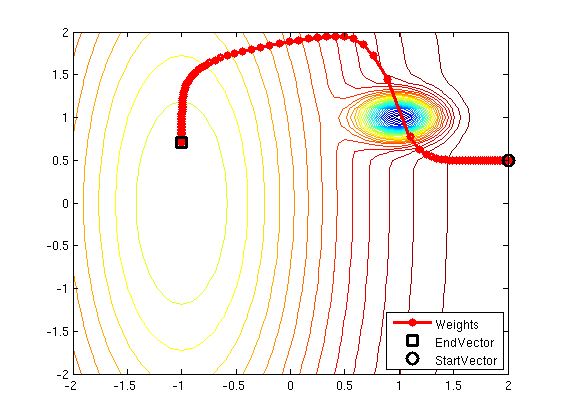
\includegraphics[width=0.8\textwidth]{./figures/212/path_w01_eta02.png}
  \caption{Verlauf von $\vect{w}$}
  \label{fig:impulse_path_w01_eta02}
\end{figure}

\begin{figure}[h!]
  \centering
  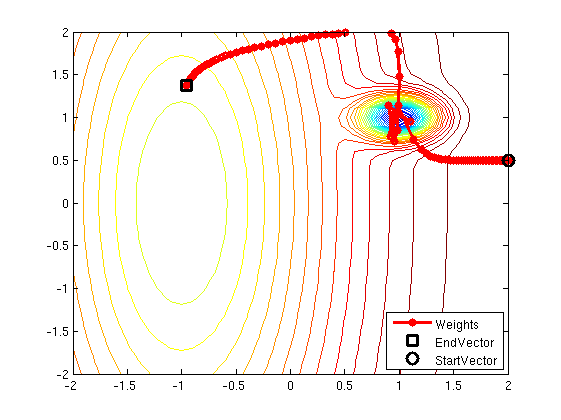
\includegraphics[width=0.8\textwidth]{./figures/212/path_w01_eta015.png}
  \caption{Verlauf von $\vect{w}$}
  \label{fig:impulse_path_w01_eta015}
\end{figure}

\begin{figure}[h!]
  \centering
  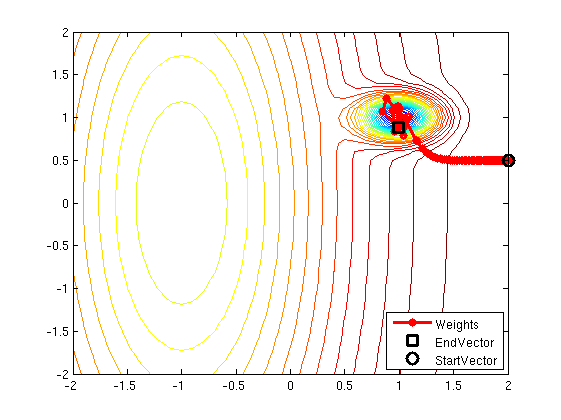
\includegraphics[width=0.8\textwidth]{./figures/212/path_w01_eta01.png}
  \caption{Verlauf von $\vect{w}$}
  \label{fig:impulse_path_w01_eta01}
\end{figure}

\begin{figure}[h!]
  \centering
  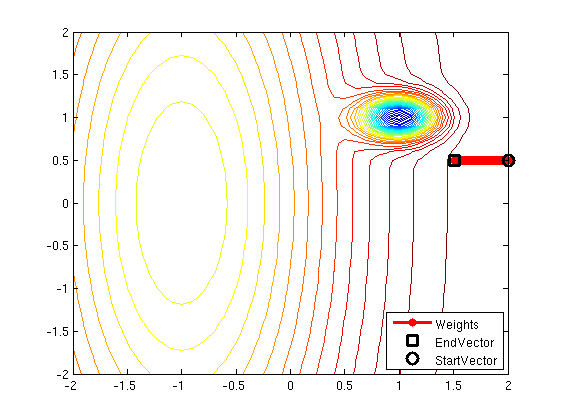
\includegraphics[width=0.8\textwidth]{./figures/212/path_w01_eta005.png}
  \caption{Verlauf von $\vect{w}$}
  \label{fig:impulse_path_w01_eta005}
\end{figure}

\begin{figure}[h!]
  \centering
  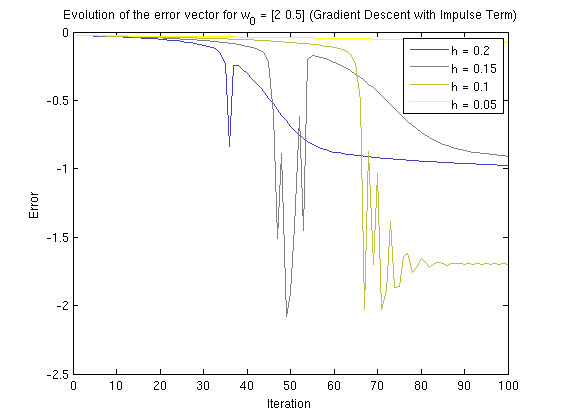
\includegraphics[width=0.8\textwidth]{./figures/212/error_w01.png}
  \caption{Verlauf von $f(\vect{w})$}
  \label{fig:impulse_error_w01}
\end{figure}

\begin{figure}[h!]
  \centering
  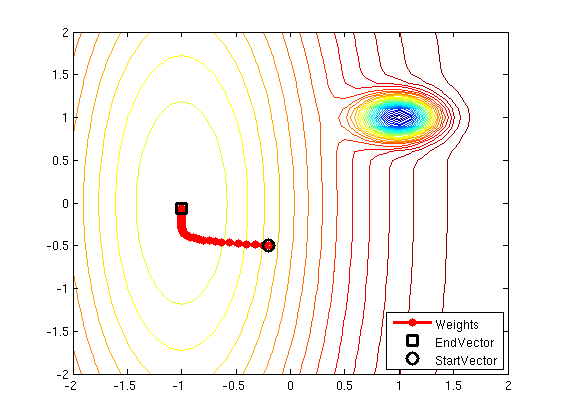
\includegraphics[width=0.8\textwidth]{./figures/212/path_w02_eta02.png}
  \caption{Verlauf von $\vect{w}$}
  \label{fig:impulse_path_w02_eta02}
\end{figure}

\begin{figure}[h!]
  \centering
  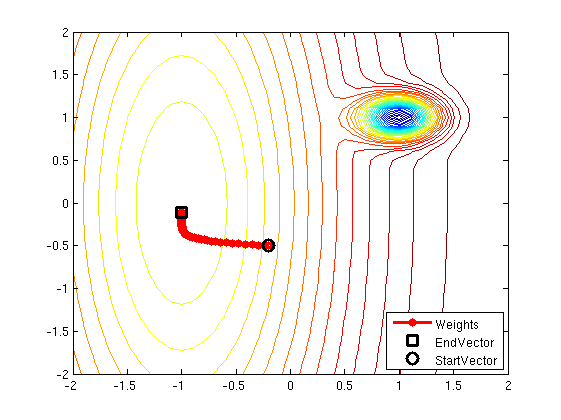
\includegraphics[width=0.8\textwidth]{./figures/212/path_w02_eta015.png}
  \caption{Verlauf von $\vect{w}$}
  \label{fig:impulse_path_w02_eta015}
\end{figure}

\begin{figure}[h!]
  \centering
  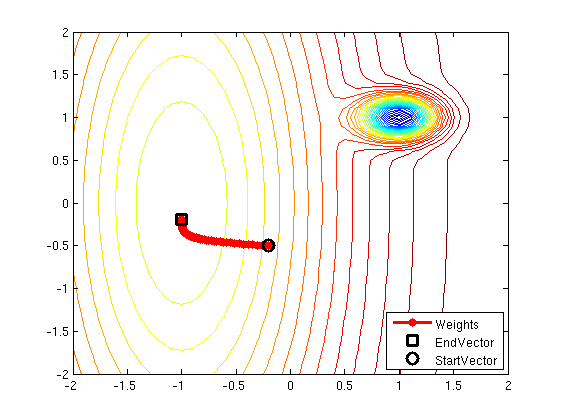
\includegraphics[width=0.8\textwidth]{./figures/212/path_w02_eta01.png}
  \caption{Verlauf von $\vect{w}$}
  \label{fig:impulse_path_w02_eta01}
\end{figure}

\begin{figure}[h!]
  \centering
  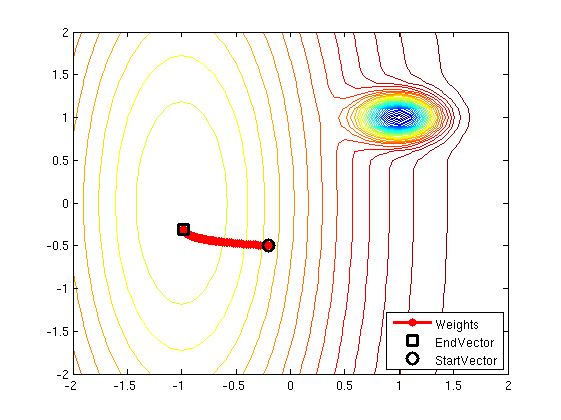
\includegraphics[width=0.8\textwidth]{./figures/212/path_w02_eta005.png}
  \caption{Verlauf von $\vect{w}$}
  \label{fig:impulse_path_w02_eta005}
\end{figure}

\begin{figure}[h!]
  \centering
  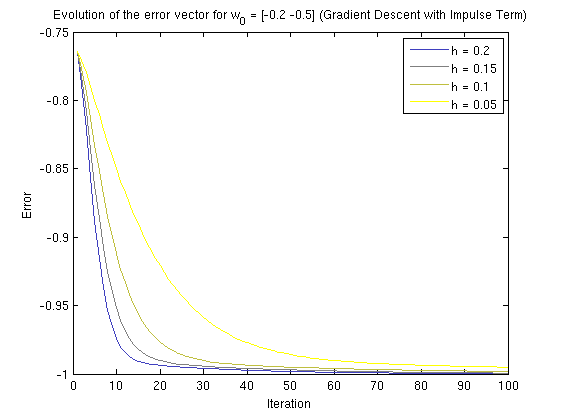
\includegraphics[width=0.8\textwidth]{./figures/212/error_w02.png}
  \caption{Verlauf von $f(\vect{w})$}
  \label{fig:impulse_error_w02}
\end{figure}

\clearpage

